\documentclass[12pt]{article}

\usepackage{booktabs}
\usepackage[margin=1in]{geometry}
\usepackage{array}
\usepackage{multirow}
\usepackage{caption}
\usepackage[usenames,dvipsnames]{xcolor}
\usepackage{amsmath}
\usepackage{amsfonts}
\usepackage{newtxtext,newtxmath}
\usepackage{inconsolata}
\usepackage[style=ieee, url=false, eprint=false, doi=true]{biblatex}
\usepackage{hyperref}
\usepackage{graphicx}
\usepackage{sidecap}
\usepackage{enumitem}
\usepackage{xfrac}
\usepackage{xcolor}
\usepackage{authblk}
\usepackage{pdflscape}
\usepackage{mhchem}
\usepackage{subcaption}
\usepackage[T1]{fontenc}
\usepackage{listings}

\lstdefinestyle{pythonstyle}{
    language=Python,
    basicstyle=\ttfamily\footnotesize,
    keywordstyle=\color{RoyalPurple},
    commentstyle=\color{teal}\itshape,
    stringstyle=\color{Maroon},
    numberstyle=\tiny\color{gray},
    numbers=left,
    numbersep=6pt,
    showstringspaces=false,
    breaklines=true,
    frame=single,
    framerule=0.3pt,
    rulecolor=\color{gray!50},
    xleftmargin=1.5em,
    aboveskip=0.5em,
    belowskip=0.5em,
}

\hypersetup{
  colorlinks   = true, % colors links instead of ugly boxes
  citecolor    = teal, % default is light green, not very legible
  linkcolor    = RoyalPurple
}

\title{MAE6760 Final Project \\ Prey State Estimation for Dragonfly Hunting}
\author{Jean Pecquet}
\date{}

\bibliography{refs}

\begin{document}

\maketitle

\vspace{-1cm}
\begin{figure}[h!]
    \centering
    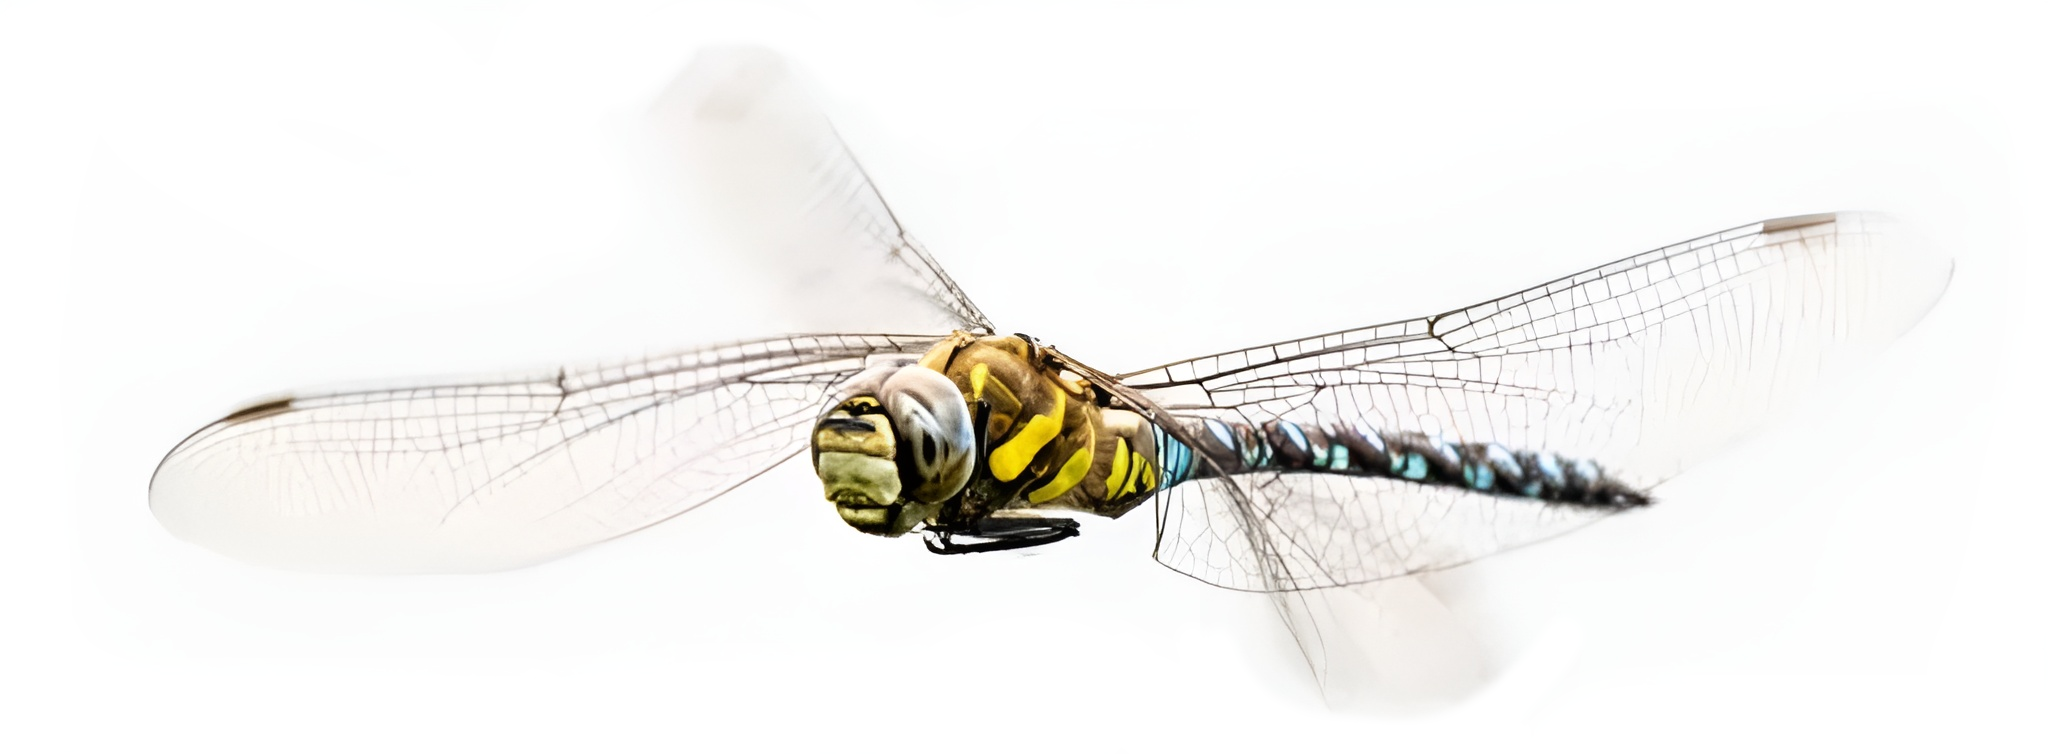
\includegraphics[width=0.7\textwidth]{dragonfly.png}
\end{figure}
\vspace{-1cm}

\section{Motivation}

Dragonfly pursuit dynamics is a highly complex problem
involving unsteady aerodynamics, control theory, and neurobiology.
While the wing kinematics leading to prey capture can be
observed with high-speed cameras, there remains significant
uncertainty as to how the wing muscle commands are formulated
based on the available sensory inputs. Some evidence suggests
that dragonflies use predictive models of prey behavior to
better anticipate prey motion \cite{mischiati2015}. This would
be much more sophisticated than other invertebrate predators like tiger
beetles, which appear to use simple proportional control
of turn rate based on the angular position of the prey in the field
of view \cite{haselsteiner2014}. In this study, we introduce a
simplified model of dragonfly flight dynamics, and develop
a model-based estimation approach for interception of a passive
prey with a prescribed trajectory. We compare the results of this
approach with a simple proportional control law.

\section{Model Description}

\subsection{Setup and Coordinates}

Real insect flight is very much a three-dimensional problem,
and involves body rotations about all three axes.
The flight dynamics are made very complex by the
strong coupling between wing motion and body pitch and roll,
which leads to interesting questions about stability, see e.g. \cite{wang2026}.
Here, for simplicity, we liken our insects to point masses,
and confine their motion to the $(x,z)$ plane, where
$x$ is parallel to the ground, and $z$ is normal to the ground,
so as to capture the influence of gravity. The resulting
motion only has 2 degrees of freedom. In the hunting setup,
the prey follows a prescribed motion,
and the dragonfly maneuvers to pursue and capture it. In our
simple model, the prey does not attempt an escape, in fact it
does not react to the dragonfly at all. We go on to describe
the dragonfly and prey models.

\subsection{Dragonfly Model}

We model the dragonfly as a point mass subjected to the force of
gravity and to the aerodynamic forces developed by its two
pairs of flapping wings. The body motion is 2D, but the wing motion
is 3D, and assumed to be symmetrical about the $(x,z)$ plane
(left and right wing motion is identical) such that there are
no lateral-directional moments and no sideforce. Any pitch
moment that would occur in reality due to the inevitable
offset between the instantaneous centers of mass and pressure
is neglected. This simplification removes an important constraint
on the wing kinematics, which is to produce the desired pitch moment
(zero over a cycle for steady flight, nonzero for maneuvers).
Their only responsibility in our model is to produce the desired body
acceleration. With this simplified model, we can write the dragonfly
state as $\xi = [x, z, \dot{x}, \dot{z}]^T$.

\subsubsection{Aerodynamic Force Model}

A major challenge of insect flight modeling is the very complex
aerodynamics. Almost the entire range of possible angles of
attack may be covered over a single wingbeat, and the reciprocating
nature of the motion causes the wings to be strongly affected by
their own wakes and those of their neighbors.
Here the wings are modeled as flat plates, divided along the span
direction into small elements, such that any area distribution
can be applied. Lift and drag forces are evaluated at each element.
First the relative velocity of the air is projected onto a plane normal
to the span direction. Then the angle of attack is evaluated
and a simple model for the all-attitude lift and drag
coefficients is used:
\begin{align}
    C_D(\alpha) &= 1.4 - \cos{2\alpha} \\
    C_L(\alpha) &= 1.2 \sin{2\alpha}
\end{align}
This model, based on Newtonian theory, is due to \cite{wang2004} and
was found to be a workable approximation when compared to experiments,
even though it completely neglects a plethora of aerodynamic phenomena,
including wing-wing interactions. The contributions of each wing element
are then summed to obtain the resultant force on the body.

\subsubsection{Wing Kinematics}

The wing orientation can be described by 4 angles: $\gamma$, the stroke plane angle,
$\beta$, the coning or sweep angle, $\varphi$, the stroke or flapping angle, and $\psi$,
the feathering or pitch angle. We will not cover the mathematical formulation
in detail. Instead we offer a graphical representation which hopefully makes
the definitions of these angles clear. Briefly: $\gamma$ describes the orientation
of the plane traced by the wing tips over a cycle, relative to the horizontal.
$\gamma$ is variable, albeit on a longer time scale than the wingbeat.
$\beta$ is the angle between the span axis and the stroke plane, and is analogous
to the sweep angle in aviation. We take it to be constant and equal to 0. Dragonfly forewings
usually have a small forward sweep, and hindwings have a small backward sweep,
with negligible effects on the aerodynamic force.
$\varphi$ and $\psi$ describe the wing motion within the stroke plane, and
are prescribed by sinusoidal functions of time. To limit the number of parameters,
we assume that the motion of the forewings and hindwings is identical save for
some phase shift $\sigma_0$. The phase shift between feathering and stroke is $\delta_0$.
\begin{align}
    \varphi_\text{fw}(t) &= \varphi_1 \cos{(\omega_0 t)} \\
    \varphi_\text{hw}(t) &= \varphi_1 \cos{(\omega_0 t + \sigma_0)} \\
    \psi_\text{fw}(t) &= \psi_0 + \psi_1 \cos{(\omega_0 t + \delta_0)} \\
    \psi_\text{hw}(t) &= \psi_0 + \psi_1 \cos{(\omega_0 t + \delta_0 + \sigma_0)}
\end{align}

\begin{figure}[h!]
    \centering
    \captionsetup[subfigure]{skip=1pt}
    \begin{subfigure}[t]{0.49\textwidth}
        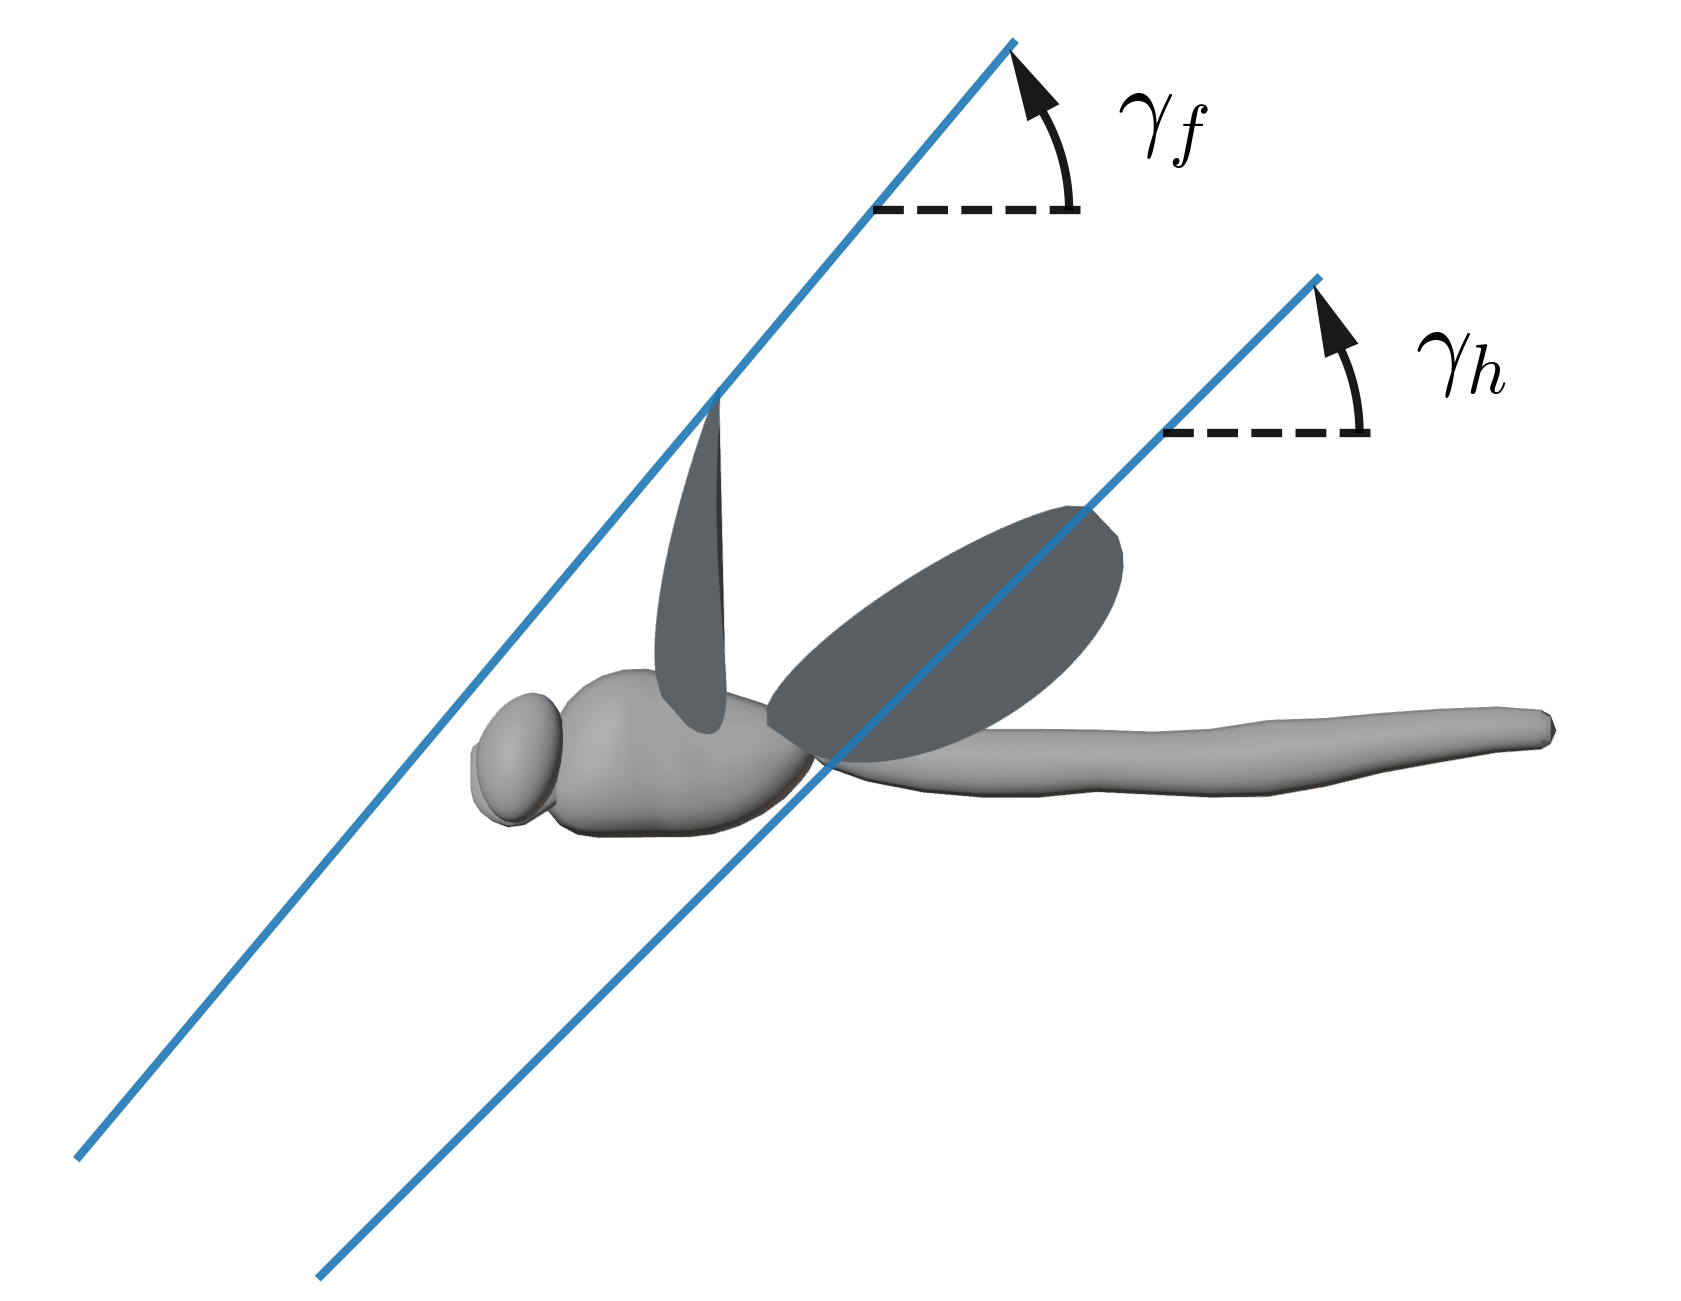
\includegraphics[width=\linewidth]{gamma.png}
    \end{subfigure}\hfill
    \begin{subfigure}[t]{0.49\textwidth}
        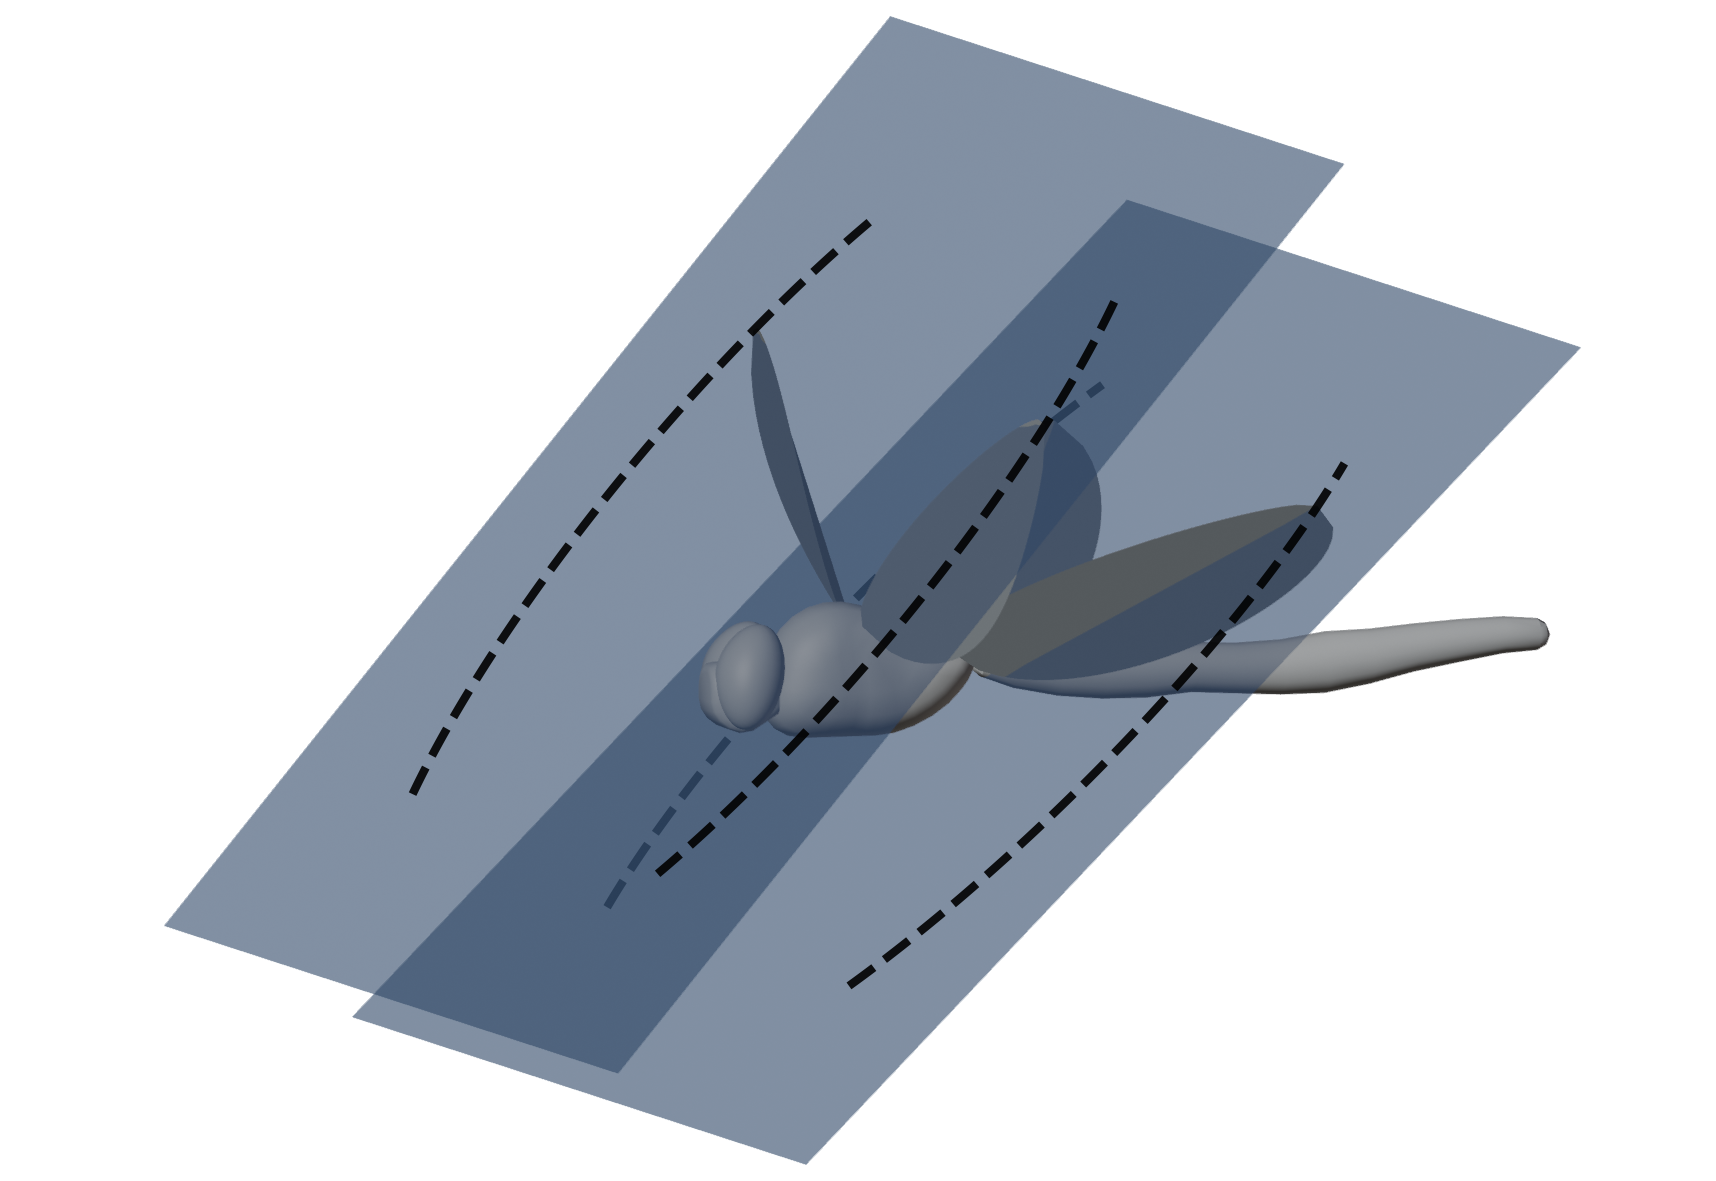
\includegraphics[width=\linewidth]{stroke-plane.png}
    \end{subfigure}

    \vspace{1pt}
    \begin{subfigure}[t]{0.49\textwidth}
        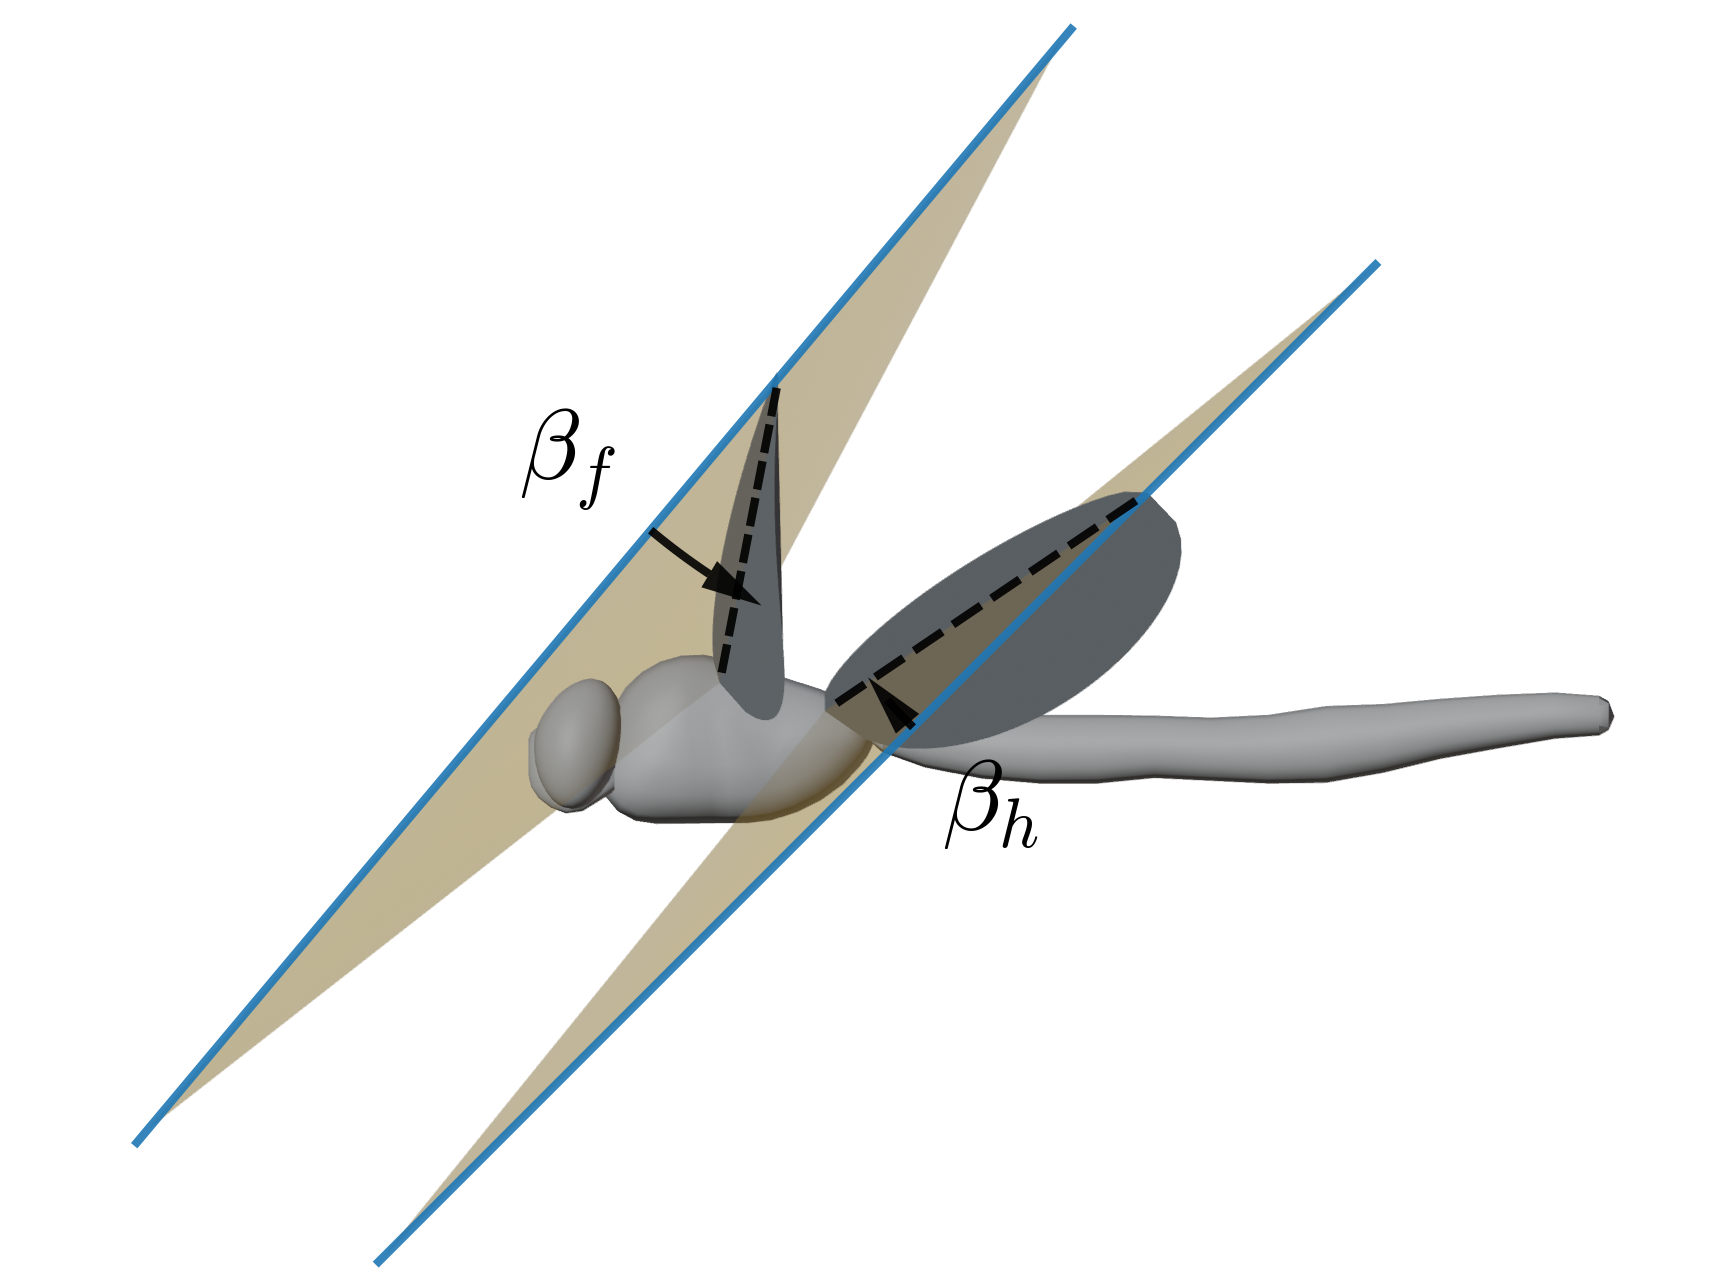
\includegraphics[width=\linewidth]{beta.png}
    \end{subfigure}\hfill
    \begin{subfigure}[t]{0.49\textwidth}
        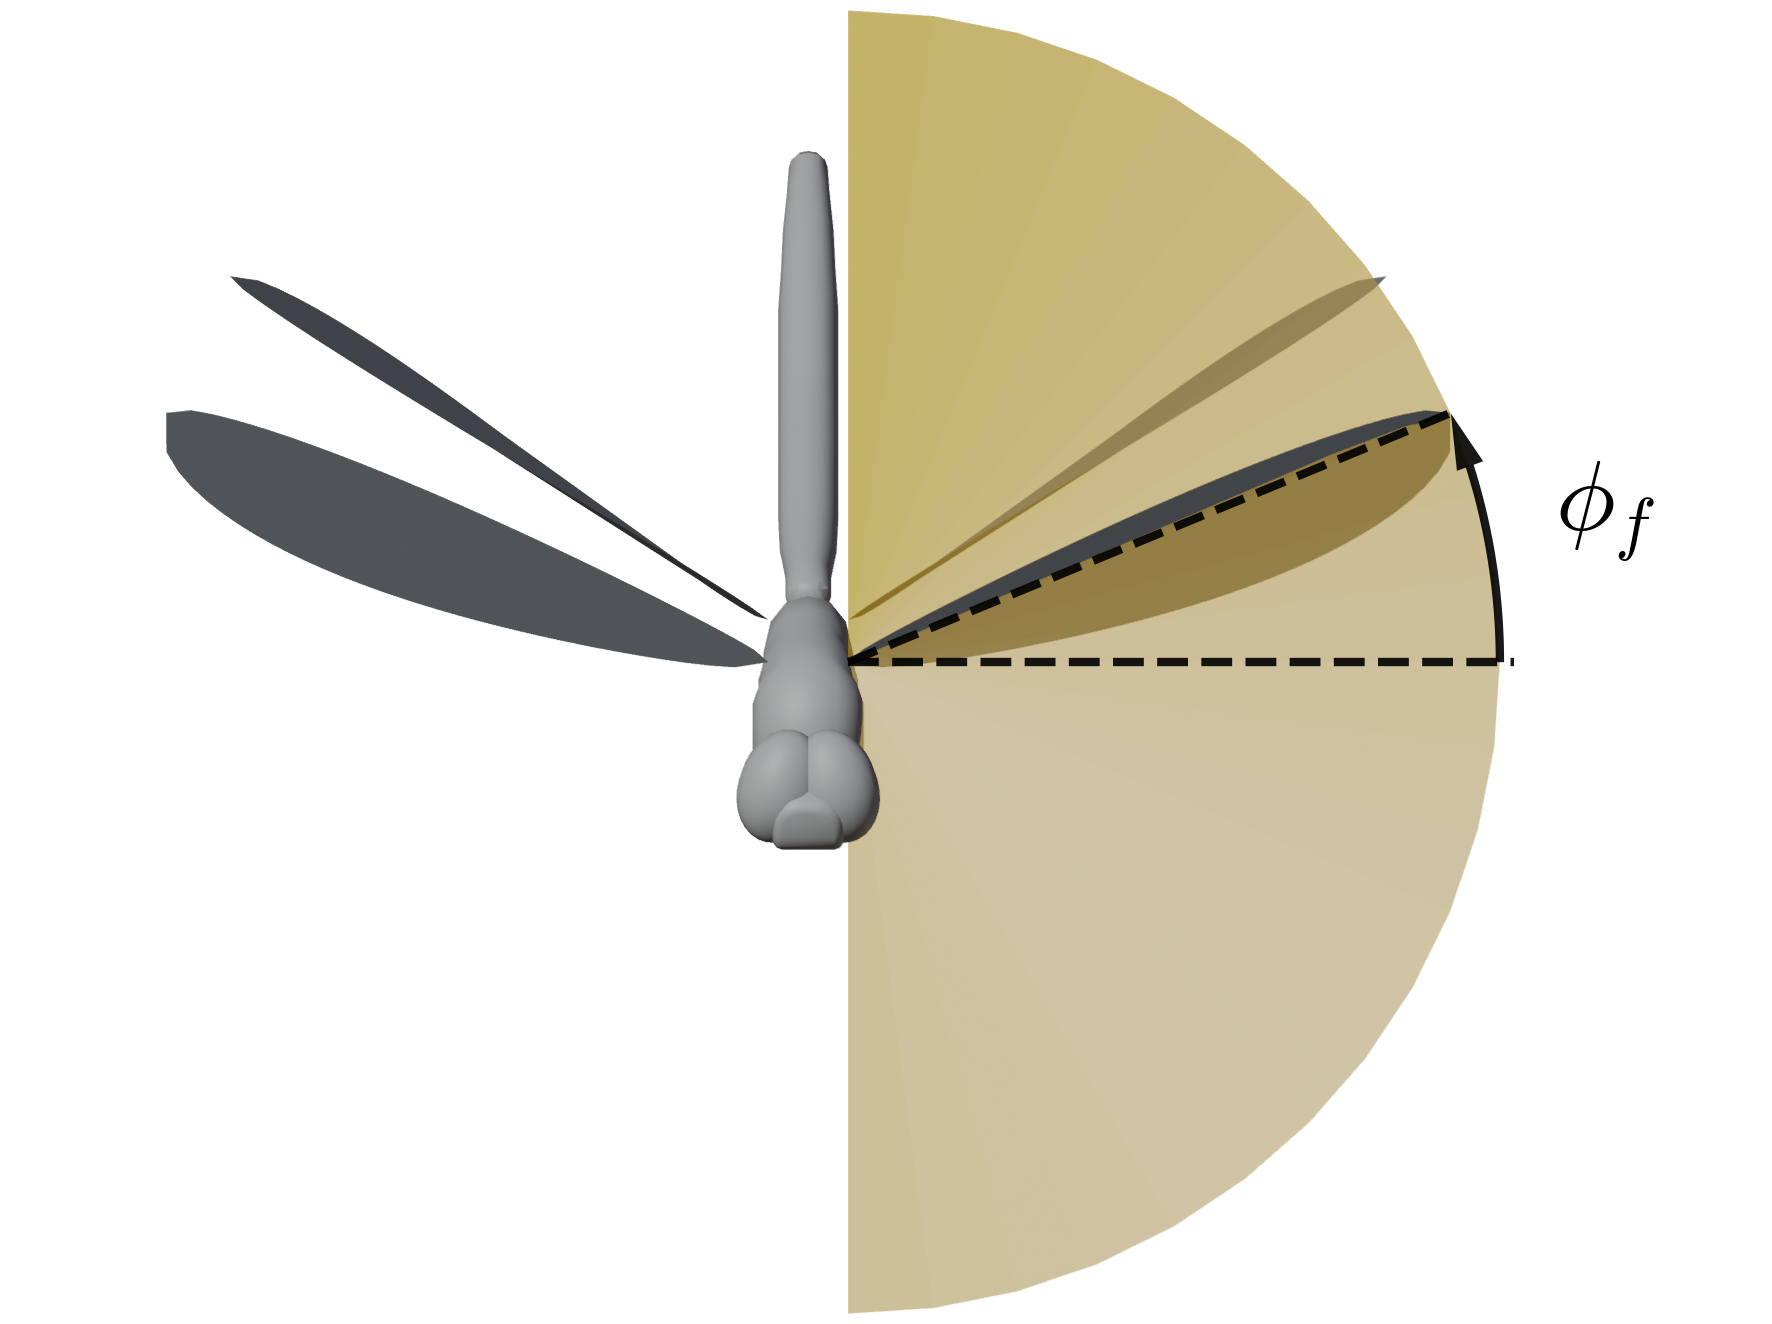
\includegraphics[width=\linewidth]{phi.png}
    \end{subfigure}

    \vspace{1pt}
    \begin{subfigure}[t]{0.85\textwidth}
        \centering
        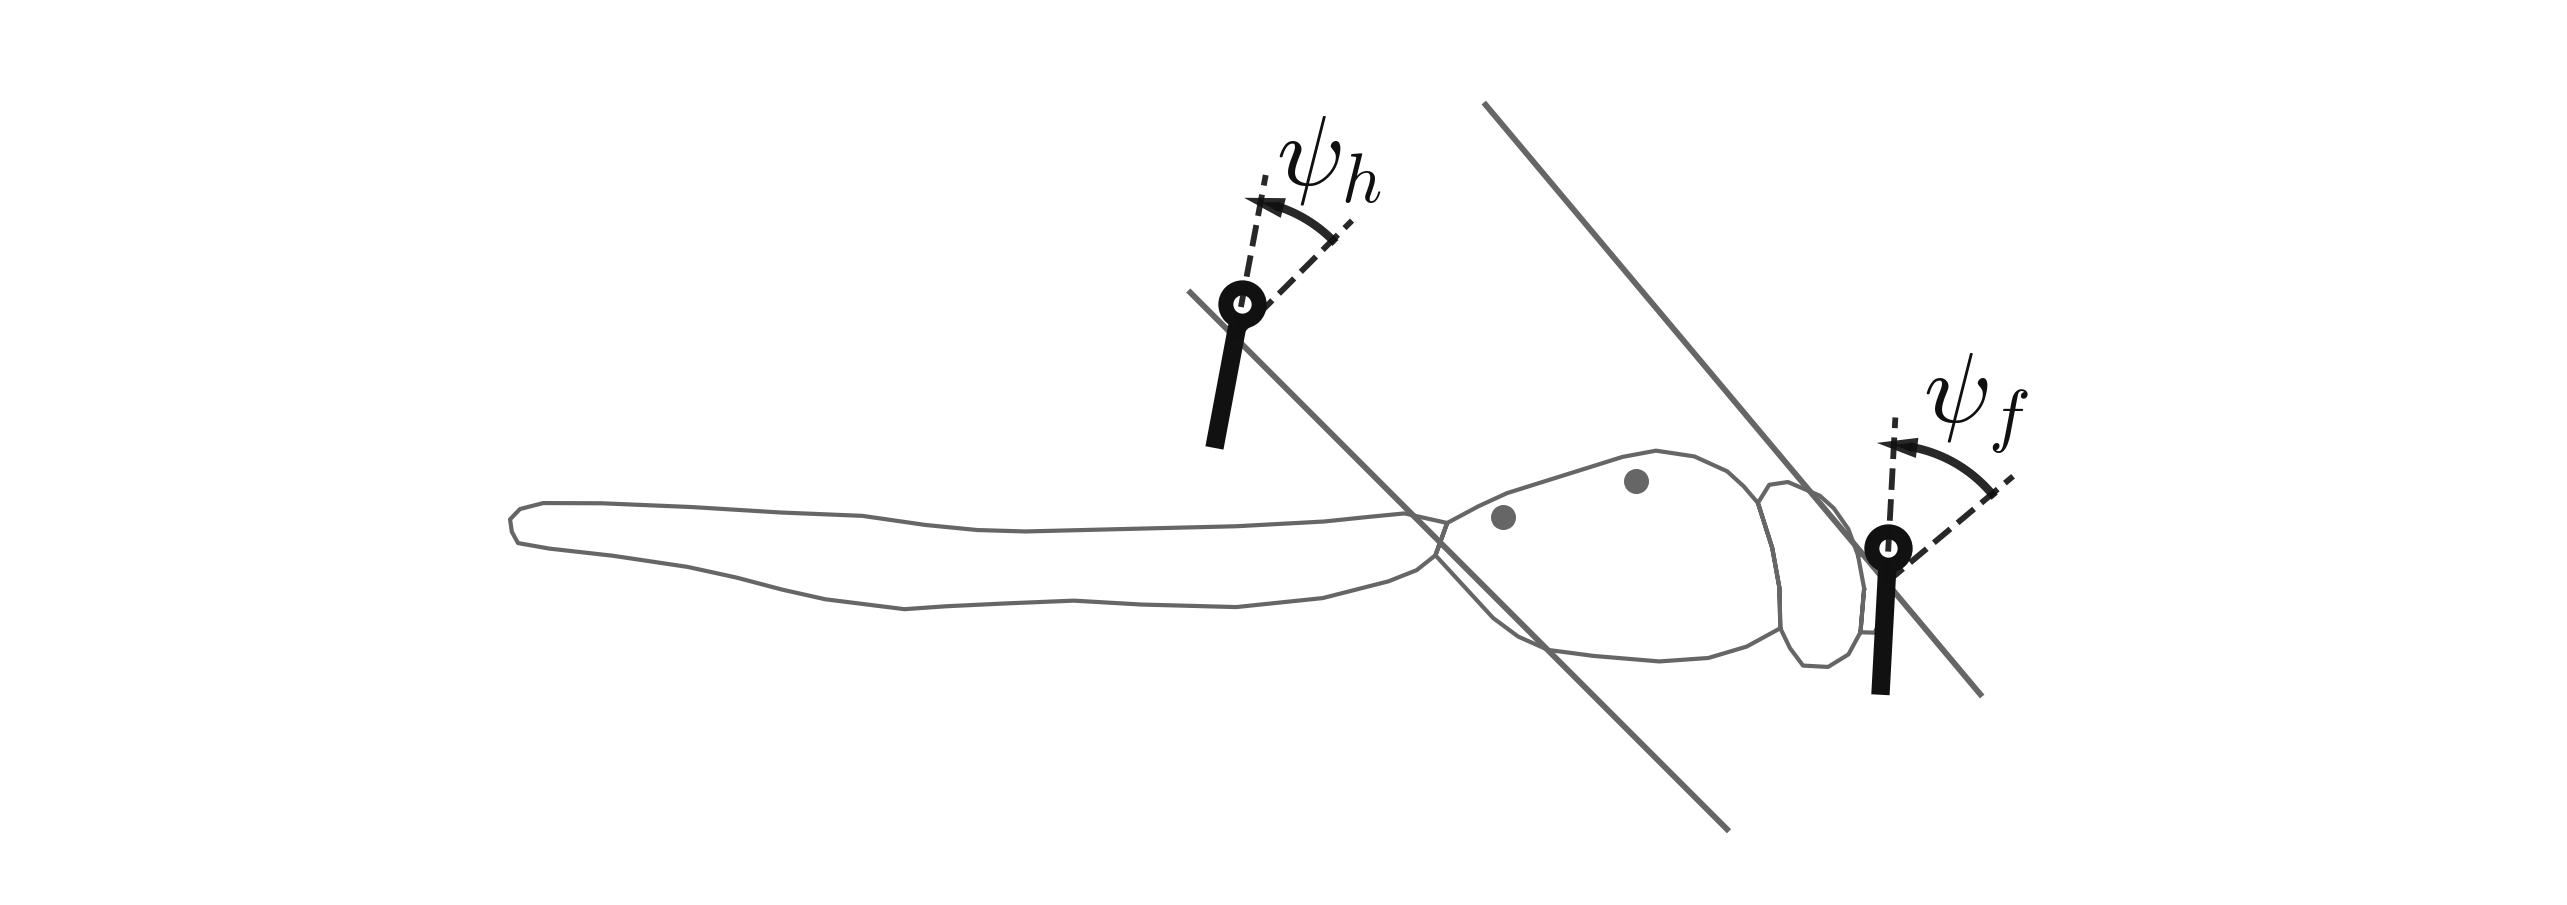
\includegraphics[width=\linewidth]{psi.png}
    \end{subfigure}
\end{figure}

\subsubsection{Non-dimensionalization}

We find it convenient to nondimensionalize the dynamics equation.
We choose the dragonfly body length $L_b$ as the length scale, and use
gravitational acceleration $g$ to define the time scale as $\mathcal{T} = \sqrt{L_b / g}$.
Three nondimensional numbers emerge from this process:
\begin{itemize}
    \item $\omega_0^* = \omega_0 \sqrt{\frac{L_b}{g}} \quad$: the nondimensional wing beat frequency
    \item $\mu_0^* = \frac{\rho_\text{air} S L_b}{m} \quad$: the nondimensional wing loading, where $S$ is the planform area of one wing, and $m$ is the total mass
    \item $\lambda_0^* = L_w / L_b \quad$: the nondimensional wing length
\end{itemize}
In general, the fore- and hindwings may have different values
of $\mu_0^*$ and $\lambda_0^*$, but here we assume they have
identical geometries. From literature on dragonfly morphology \cite{wakeling1997},
we find that representative values of the nondimensional parameters
are $\omega_0^* = 4\pi$, $\mu_0^* = 0.075$, and $\lambda_0^* = 0.75$.
We use these as a baseline.

\subsection{Prey Model}

We make no attempt to model the aerodynamics of the prey. Instead, we
prescribe its motion using a constant-velocity model with white
process noise. Taking the prey state to be $\xi_p = [x_p, z_p, \dot{x}_p, \dot{z}_p]^T$,
the dynamics are:
\begin{align}
    \ddot{x}_p &= w_x \\
    \ddot{z}_p &= w_z
\end{align}
where $w_x$ and $w_z$ are independent zero-mean Gaussian processes with
(nondimensionalized) intensity $q_p^*$. With small $q_p^*$ we approach
the deterministic constant-velocity case,
while large $q_p^*$ makes the trajectory effectively unpredictable beyond a
short horizon. We use this same model both to generate the true prey
trajectories and as the internal model the dragonfly uses for estimation.

\section{Controller Design With and Without State Estimation}

\subsection{Without State Estimation}

For pursuit, given our 2D model, we are primarily concerned with
the velocity heading angle $\theta$. The most intuitive control
variable for $\theta$ is the stroke plane angle $\gamma$, since for
a symmetric wing stroke (wing pitch angle $\psi$
during the downstroke is the opposite of what it is
during the upstroke, i.e. $\psi_0 = 0$), the aerodynamic
force direction is normal to the stroke plane. In our design, the
wing flapping and pitching amplitudes $\varphi_1$ and $\psi_1$
are fixed to provide high acceleration and a high speed ceiling,
and $\dot\gamma$ obeys a proportional control law analogous to the
tiger beetle turn rate control law from \cite{haselsteiner2014}:
\begin{equation}
    \dot\gamma(t) = -K \theta_e(t - \tau)
\end{equation}
where $K$ is a proportional gain, $\theta_e = \theta_p - \theta$
in which $\theta_p$ is the prey bearing, and $\tau$ is the
muscle chain delay between the brain issuing a command and the wings
actually executing it, which we take to be half a wingbeat
($\tau/T_{wb} = 0.5$). The compound eye perceptual delay is neglected.
Note that while the stroke plane angle is a mode of directional
control for dragonflies, it is only secondary compared to
body pitch. Since the current model is a simple 2 DoF model,
we can consider $\gamma$ to stand in for both stroke plane tilt
and body pitch, since the actual mechanics behind body pitch
(complex, due to wing moments) are obscured.

\subsection{With State Estimation}

In principle, a disadvantage of the proportional control law
is that the dragonfly does not anticipate the prey motion,
and always steers towards the prey's current bearing.
By estimating the prey's state, and converting that estimate
into a bearing, the prey capture performance may be improved
(by metrics we have yet to define).

\subsubsection{Prey State Estimation}

We use an extended Kalman filter (EKF) on the prey state $\xi_p$,
propagating it forward under the same constant-velocity model
with white-noise acceleration used to generate the trajectory.
We assume that the dragonfly is able to keep track of its own
state $\xi$ using a variety of sensory organs.
The compound eye delivers a noisy prey bearing $y_\theta$ to the nervous system
\begin{equation}
    y_\theta = \arctan{\frac{z_p - z}{x_p - x}} + v_\theta,
    \qquad v_\theta \sim \mathcal{N}(0, R_\theta),
\end{equation}
This is nonlinear in $\xi_p$, so we linearize about the current mean
at each update step. The filter is initialized with a prior
$\hat\xi_p(0) \sim \mathcal{N}(\bar\xi_p, P_0)$.
To improve observability, we may want to include information
on the apparent size of the prey into the estimate. We will discuss this
further in the Results section.

\subsubsection{Lead Pursuit}

From the estimated prey state and the dragonfly's own state, we
compute a lead point. That is, the point where the prey is predicted to be when
the dragonfly catches it, assuming the prey continues at its
currently-estimated velocity $\hat v_p$ and the dragonfly travels at
its current speed $v$ in a straight line. The time-to-go
$t_\text{go}$ verifies
\begin{equation}
    \lvert \hat r + \hat v_p\, t_\text{go} \rvert
    = v \, t_\text{go},
\end{equation}
where $\hat r = \hat p_p - p$ is the estimated relative position.
This is a quadratic in $t_\text{go}$ with a positive root whenever
the dragonfly is fast enough to ever catch the prey. The lead point is then
$\hat p_p + \hat v_p\, t_\text{go}$, and the reference bearing
$\theta_\ell$ is the angle to that point as seen from the dragonfly.
The control law is otherwise identical to simple proportional control
\begin{equation}
    \dot\gamma(t) = -K \theta_e^\text{lead}(t - \tau).
\end{equation}
Where $\theta_e^\text{lead} = \theta_\ell - \theta$.
The model-based controller differs from the proportional one
only in what bearing it aims for.
If there is no valid solution for $t_\text{go}$,
i.e. the prey moves directly away faster than the dragonfly
can chase, it falls back to pure pursuit.
\bigskip

Specific parameter values and additional improvements to the state estimate and
lead pursuit strategy will be discussed as results are presented in the
following section.

\section{Results and Discussion}

In comparing the two controllers, we would have liked to provide a
more systematic analysis of the parameter dependence of capture
rates and other success metrics over a large number of simulations.
Because of a number of issues that had to be resolved with the
existing dragonfly simulation code, as well as the lead controller
code, we present here only a limited and fairly qualitative discussion
for two representative cases.

\bigskip

We compared the two controllers for two prey trajectories: a
\textit{vertical} case where the prey climbs nearly straight up, and a
\textit{horizontal} case where the prey drifts laterally. In both, the
dragonfly starts hovering at the origin. For the vertical case the
prey appears at $(6 L_b, 0)$ with nominal velocity $(0, 1)$.
For the horizontal case the prey appears
at $(3 L_b, 3 L_b)$ with nominal velocity $(1, 0)$. The process noise
in both cases is $q_p^* = 0.1$.
Both controllers see the same prey realization within each
case. The wing stroke kinematic parameters other than the stroke
plane angle $\gamma$ are constant and selected from past studies to
provide good acceleration and a high speed ceiling. $\gamma$ is
initialized at 30$^\circ$, a value representative of dragonfly hover.
The control law gain is set to $K = 1.5$, a value considered optimal
based on previous studies of the proportional controller. The muscle
delay is set to $\tau/T_\text{wb} = 0.5$. All these parameters are
common to both the proportional and MBE controllers. The MBE filter
takes angular-size measurements with $R_\theta = 10^{-2}$, and a noisy prior $P_0 = 0.2^2 I_4$.
Capture is declared at separation $\leq 0.5 L_b$.

\begin{figure}[h!]
    \centering
    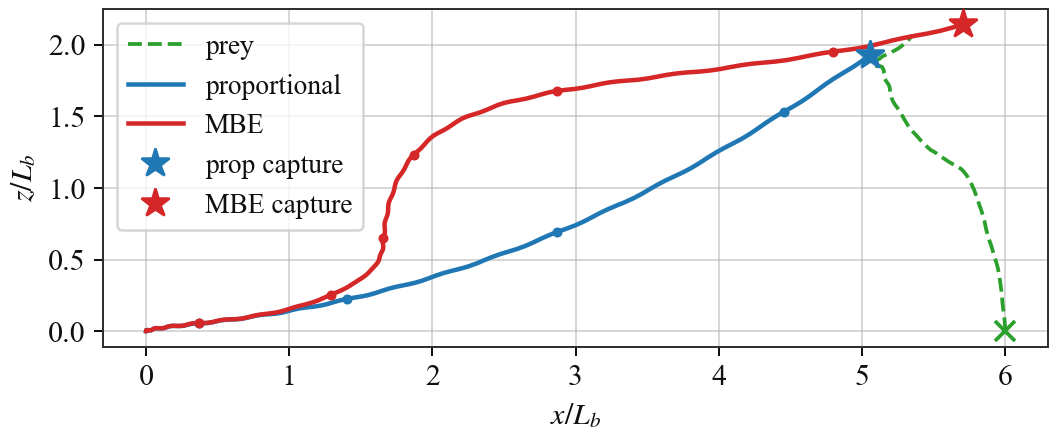
\includegraphics[width=\linewidth]{../figs/vertical_trajectories.png}
    \caption{Vertical prey trajectory}
    \label{fig:traj}
\end{figure}

\begin{figure}[h!]
    \centering
    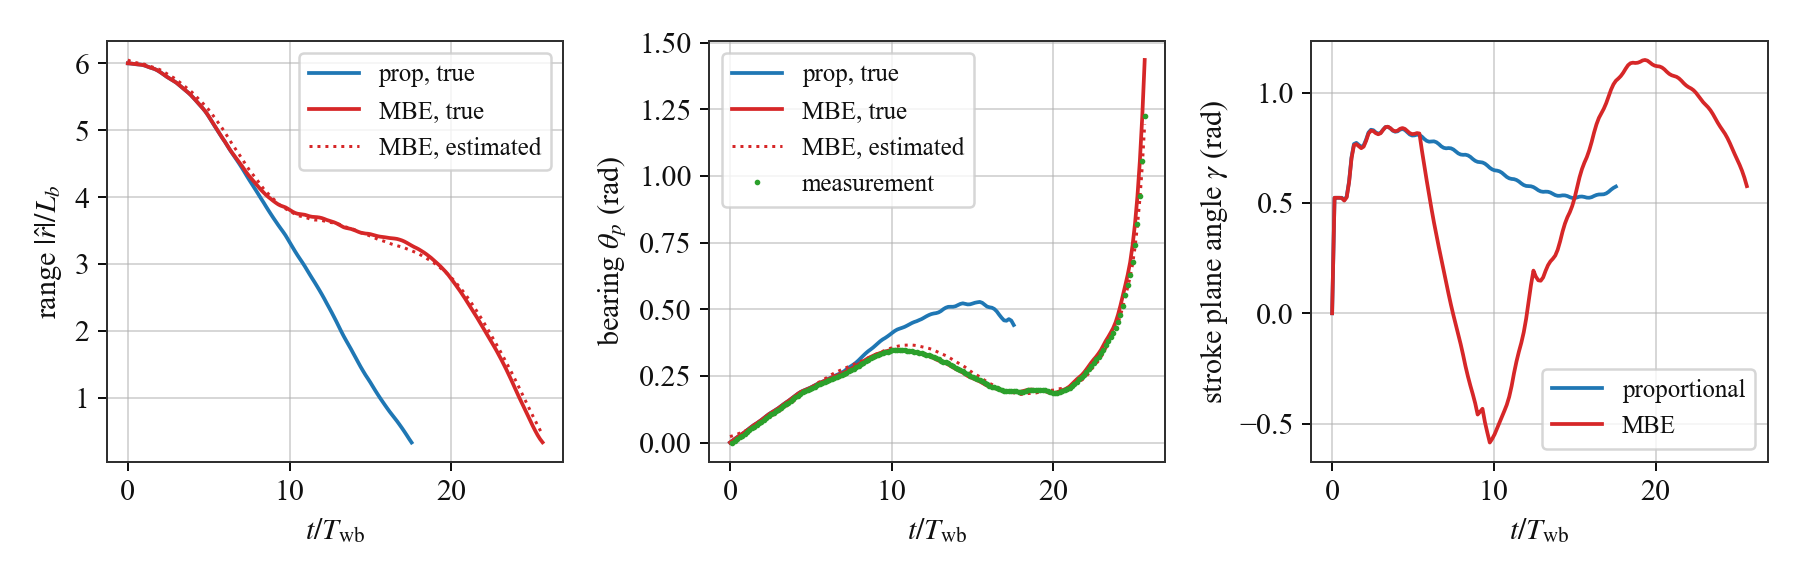
\includegraphics[width=\linewidth]{../figs/vertical_time_series.png}
    \caption{Vertical case time series}
    \label{fig:ts}
\end{figure}

It is quite obvious from the vertical case trajectories
and time traces that the MBE lead pursuit controller
does not perform as well as expected.
Both controllers capture: the proportional
controller at $t/T_\text{wb} \approx 17.5$, the MBE controller at
$25.7$, both at the capture threshold of $0.5 L_b$. The
proportional path is quite smooth. The MBE path starts off
slightly steeper as expected, but suddenly decides to pitch
up severely.
It appears that the sudden pitch up command coincides (with delay)
with a jump in the vertical velocity error. 
The dragonfly thinks the prey is a lot faster than it is,
and way overcorrects to lead its position.
Eventually the error settles a little, but remains quite
significant overall. This aside,
the estimator appears to perform reasonably well in
terms of consistency.

\begin{figure}[h!]
    \centering
    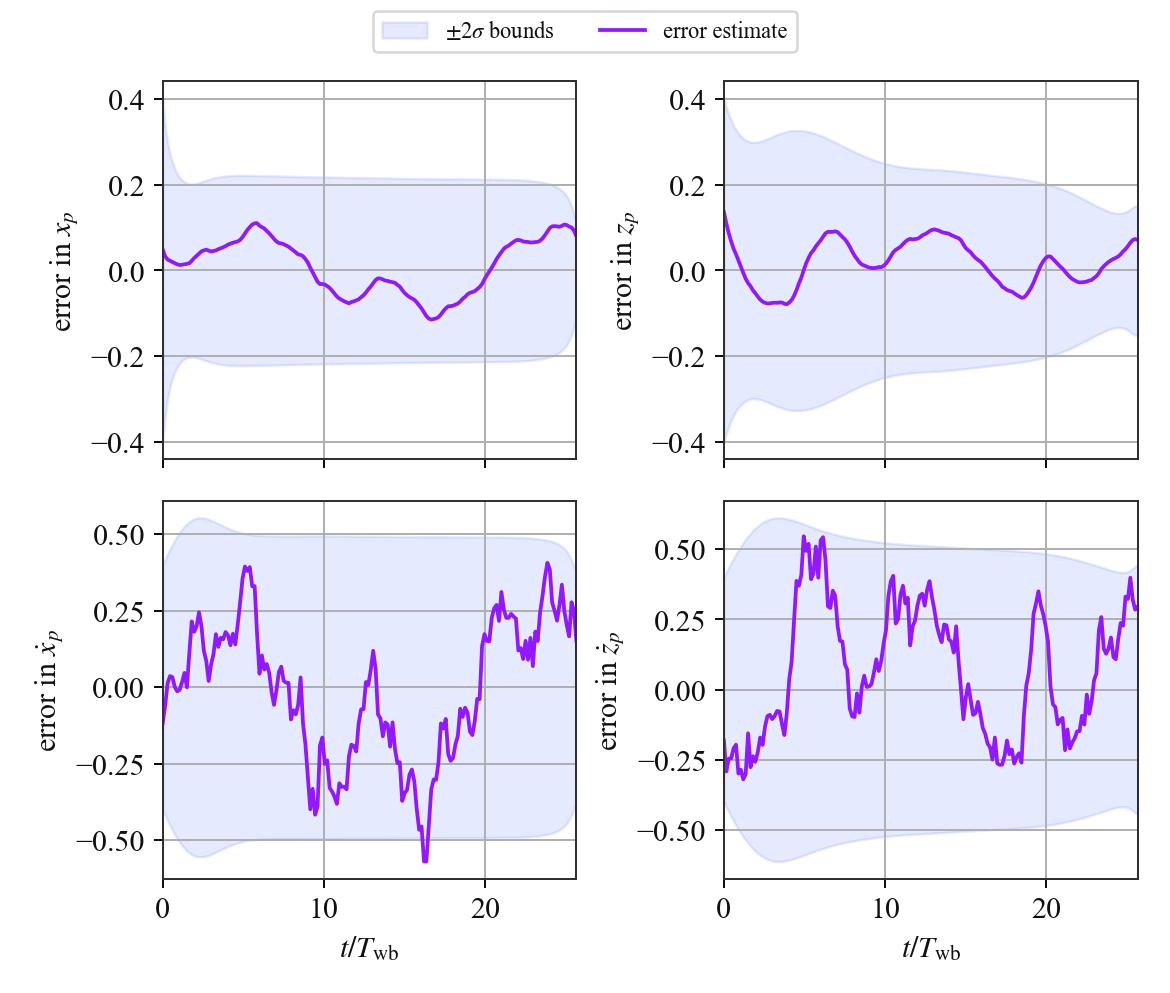
\includegraphics[width=0.82\linewidth]{../figs/vertical_filter_consistency.png}
    \caption{Vertical case estimator error}
    \label{fig:cons}
\end{figure}

The MBE controller is quite a bit more successful in the horizontal case,
and notably manages an intercept, whereas the proportional controller
is unsuccessful. In light of these two cases, it appears the MBE controller
has potential but is quite fragile. Even the dynamics of this highly
simplified dragonfly flight model are surprisingly rich,
and since the dragonfly's own state is obviously an integral part of
the prey state estimation, the dynamics can interact with the controller
in unpredictable and consequential ways.

\begin{figure}[h!]
    \centering
    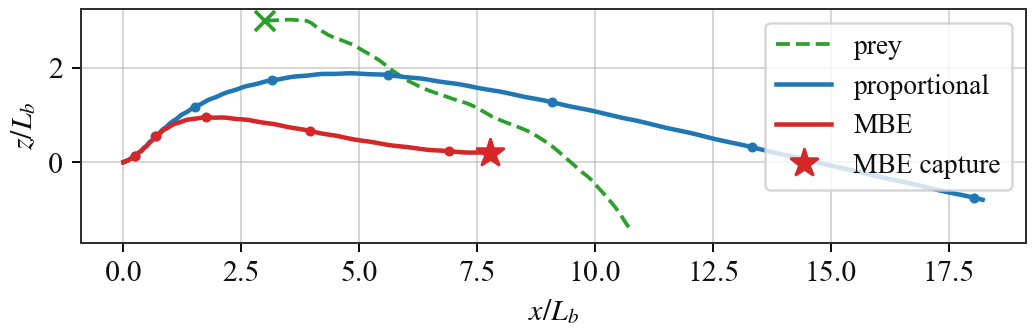
\includegraphics[width=\linewidth]{../figs/horizontal_trajectories.png}
    \caption{Horizontal prey trajectory}
    \label{fig:traj}
\end{figure}

\begin{figure}[h!]
    \centering
    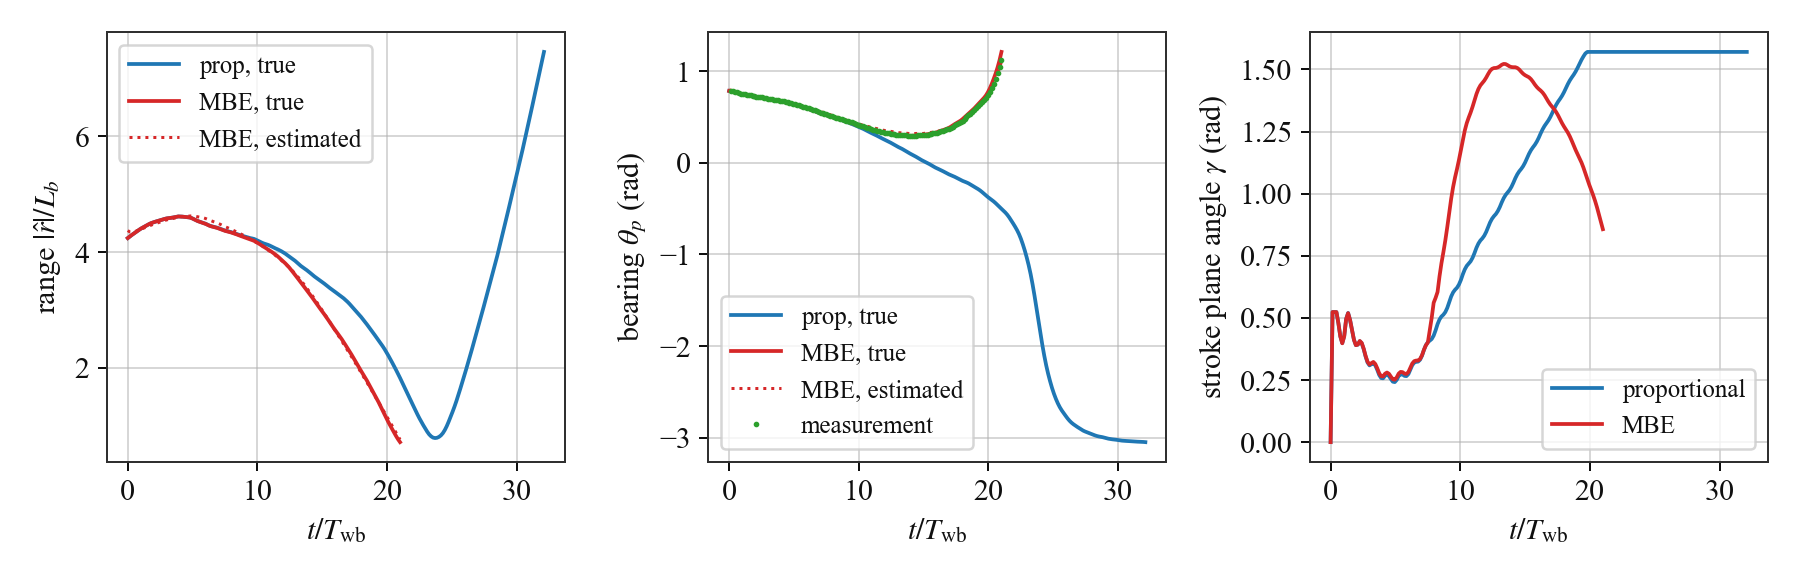
\includegraphics[width=\linewidth]{../figs/horizontal_time_series.png}
    \caption{Horizontal case time series}
    \label{fig:hts}
\end{figure}

\begin{figure}[h!]
    \centering
    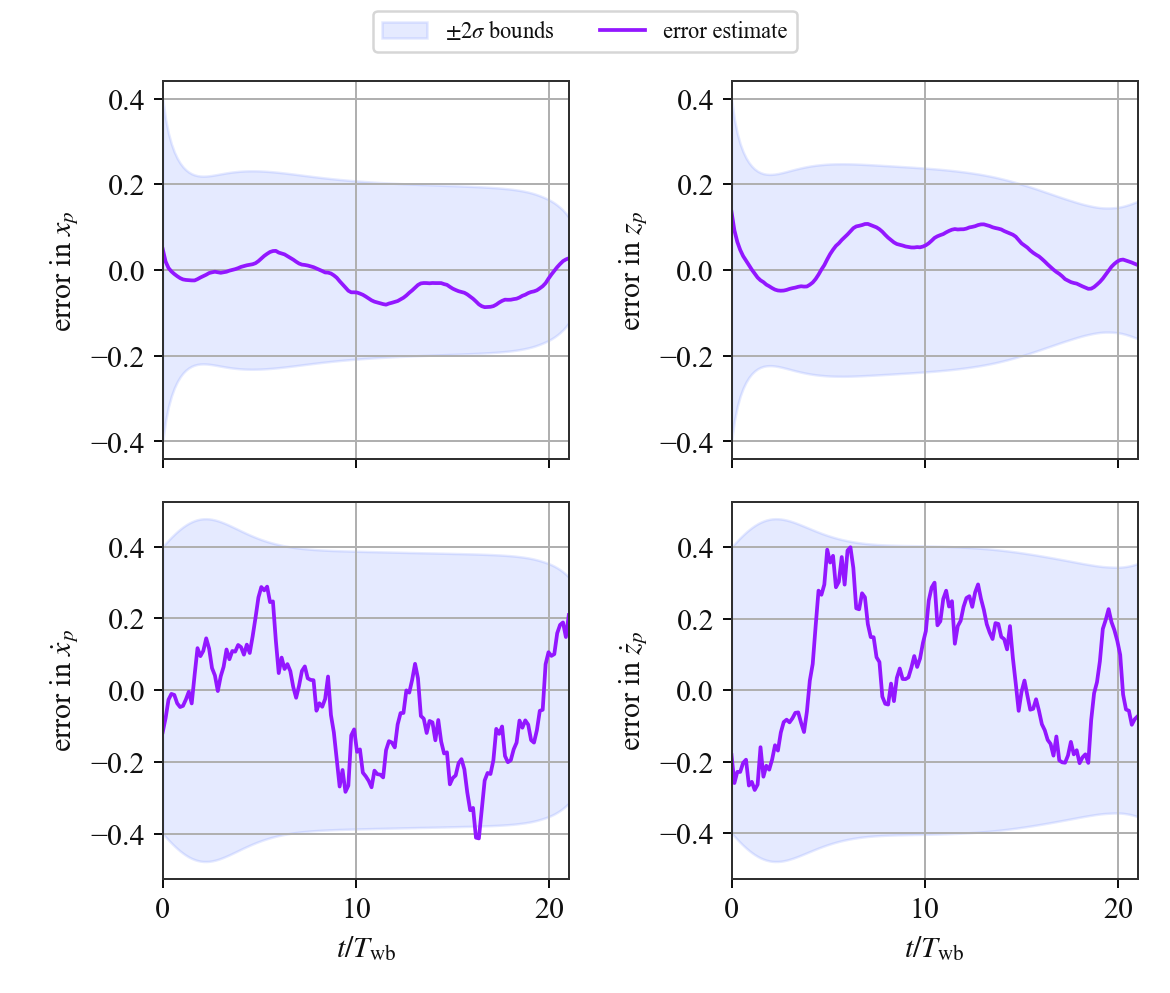
\includegraphics[width=0.82\linewidth]{../figs/horizontal_filter_consistency.png}
    \caption{Horizontal case estimator error}
    \label{fig:hcons}
\end{figure}

Since all this is hard to reason about
from first principles, an essential next step would be to conduct 
systematic sweeps of the parameter space, first for given morphology
and kinematics, then over the morphological and kinematic parameters themselves,
for a large number of simulated prey trajectories, to get a better understanding
of the controller dynamics. Since two drivers of bad performance appear to
be large estimator error and time delay, it would also make sense to think
about improving the estimate by fusing range or range rate measurements (from
angular size of prey), and somehow compensating for actuation lag within
the controller.

\printbibliography[heading=bibintoc]

%\appendix

%\section{Filter Implementation}

%\lstinputlisting[style=pythonstyle]{../../dragonpy/brain/estimator.py}

\end{document}
